\documentclass{article}
\usepackage[utf8]{inputenc}
\usepackage[english]{babel}
\usepackage{graphicx}
\usepackage{subfigure}
\usepackage{amsmath,amssymb}
\graphicspath{{images/}}

\DeclareMathOperator*{\argmin}{arg\,min}
\DeclareMathOperator{\E}{\mathbb{E}}

\title{The User Behavior On Online Judge Website}
\author{yueyi zhuo}
%\institute{School of Mathematical,Sichuan Normal University}
\date{2017}

\begin{document}

\maketitle

\begin{abstract}

Abstract content.

\end{abstract}

\section{Introduction}

In 2016 Spring Festival, I solve some problems in Project Euler 
\footnote{In fact, I solve 70+ problems before my interest fade.}, 
which may be most famous online judge 
in Internet except Leetcode. I have noticed the interesting data structure related with rank and difficulty.
But I lacked enough powerful statistic tool to process and model it. 
In fact, I model it as a ordinary least square which is not understood by me in the time. In the naive period,
linear regression model seems like a poor black box model that often be meeted in Machine Learning algorithm.

Now, partly because of study of course of Econometric, I totally understand the random model and the instance,
linear regression. 
Right, there're some random variable constrained by expectation function sharing same parameters, that's all.
A specific linear regression model correspond to many latent models specified indepent variable distribution,
but their expectation function are same. This lead to same result from estimator and model test.

My insight is given by some external user comment about their usage they use OJ. 
Someone claim that thay solve problem by order of the number of solved, but I solve problem by order of ID.
I'm fascinated by thinking that how to identify the percent of two type if we assume only the two type exists.
Since the particular problem represent a more general problem set, I would like to treat it as a bridge to that.

Let's formulate my ealiest idea, there're $N$ problems, $n$ solver. Let 
$s_{ij} \in \{ 0,1 \} \quad i \in \{ 1,\dots,n \} \; j \in \{ 1,\dots,N \}$ be whether solver $i$ solve the problem $j$.
So fixing solver $i$, we assume binary random vector $s_i = ( s_{i1} s_{i2} \dots s_{iN} )^T$ 
can be divided into some group which is determined by a specific distribution and they're independent.
Specially, I define the distribution $D_1$ which follow order of ID:


\begin{align*} % Notice align or align* is not used in math mode. They can be directly include in paragraph(normal) mode.
P(s_{i1} = 1) = p \\
P(s_{ij} = 1 | s_{i,j-1}=0) = 0 \\
P(s_{ij} = 1 | s_{i,j-1}=1) = p
\end{align*}


and define $D_2$ which follow order of the number of solved:


\begin{align*}
P(s_{i,r(1)} = 1) &= p \\
P(s_{i,r(j)} = 1 | s_{i,r(j-1)}=0) &= 0 \\
P(s_{i,r(j)} = 1 | s_{i,r(j-1)}=1) &= p
\end{align*}


in which $r(i)$ is function that map the the rank of number of solved to id
(e.g. r(10)=20 means that the rank of number of solved of 20th problem is 10).
Obviously we can replace $r(i)$ to any onther order that mean some interesting thing to get other distribution.

Let $n_1,n_2$ be the individual number that follows $D_1,D_2$, hence $n_1+n_2=n$. Unfortunately, we only can 
observe the sum of every sample sequence:

\[
S_j = \sum_{i=1}^n s_{ij}
\]

We have only data that is once obseration of statistic $S_j$ exactly. It looks like:


\begin{figure}[h]

\centering

\subfigure[Solved number series]{\label{fig:a}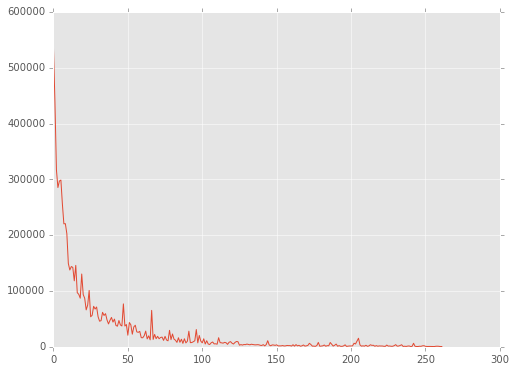
\includegraphics[width=0.49\linewidth]{solved-seq1.png}}
\subfigure[Log solved number series]{\label{fig:b}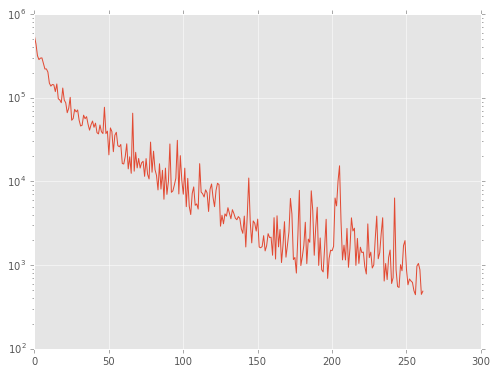
\includegraphics[width=0.49\linewidth]{solved-seq2.png}}
 
\end{figure}

The data is scraped from Project Euler \footnote{Project Euler website: https://projecteuler.net/archives }
, my problem answers, crawler program and basis analysis is hosted on GitHub \footnote{https://github.com/yiyuezhuo/euler }
This is a screenshot for Project Euler website:

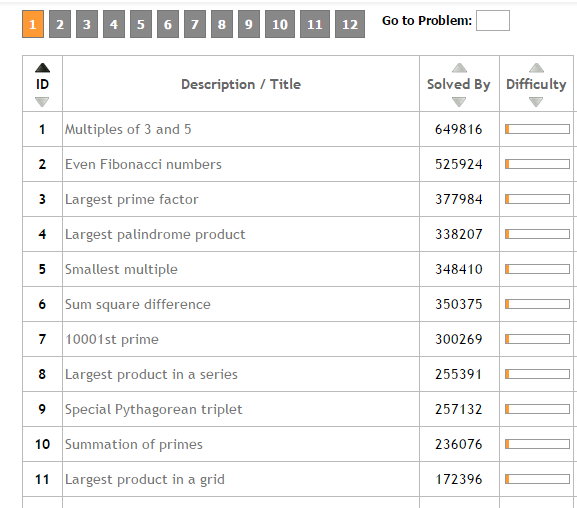
\includegraphics[scale=0.55]{euler-oj.png}

Given $n_1,n_2,p$, we can determine a model like we talk above. 
We can specify these values througn minimizing the squard loss function:

\[
\min_{n_1,n_2,p} \sum_{j=1}^N (S^*_j - \E(S_j))^2
\]

In which $S^*_j$ is real value, $S_j$ is random variable defined by model and $n_1,n_2,p$

We would like a model taking more statistic manner instead of only fitting function. 
Thus we assume that the model is \textit{real} 
\footnote{As so often happens, some funny Econometric model claim they're real, 
otherwise statistic model will reduce to awkward explore method.} 
and add a convenient noise term  $\epsilon_j$  to all $S_j$ to let our model can generate(sample) 
any possible sequence \footnote{Anyway, a pure noise model can do it too.}.

\begin{align*}
S_j = \sum_{i=1}^n s_{ij} + \epsilon_j \\
\epsilon_j \sim F \quad i.i.d 
\end{align*}

In which $F$ is a integer distribution that can take binomial distribution or something.

\[
\E(S_j) = \sum_{i=1}^n \E(s_{ij}) + \E(\epsilon_j) = \sum_{i=1}^{n_1} p^j + \sum_{i=n_1+1}^n p^{r(j)}
= n_1 p^j + n_2 p^{r(j)}
\]

and apply least expectation loss rule, very frequentist:

\[
\hat{n_1},\hat{n_2},\hat{p} = \argmin_{n_1,n_2,p} \E\sum_{j=1}^N (S_j - \hat{S_j})^2
\]

In which $\hat{S_j} = \E(S_j | \hat{n_1},\hat{n_2},\hat{p})$.

Unfortunately, this nonlinear form can't be transformed to linear form directly. Temporarily, 
we constrain $n_2 = 0$, then $n_1 = n$, then the $\E(S_j)$ reduce to:

\[
\E{S_j} = n p^j
\]

and

\[
\log \E(S_j) = \log n + j \log(p)
\]

Well, so we can estimate $n,p$ by estimating $\log(n),\log(p)$ by running ordinary least square method to 
minimize the objective function \footnote{Alrough I feel that this conversion is not strict true, since
it assign different weights on every data point.}: 

\[
\min_{\hat{n},\hat{p}} \sum_{j=1}^N ( S_j - (\log(\hat{n}) + j \log(\hat{p})) )
\]

For the real data, the estimated results are:

\[
\hat{n} = 95132.76 \quad \hat{p} = 0.98002
\]

The $\hat{n}$ looks too small and $\hat{p}$ looks too big as we notice the quick fall of sequence head that
can not be expressed the too small $\hat{p}$ as the fit graph illustrate:

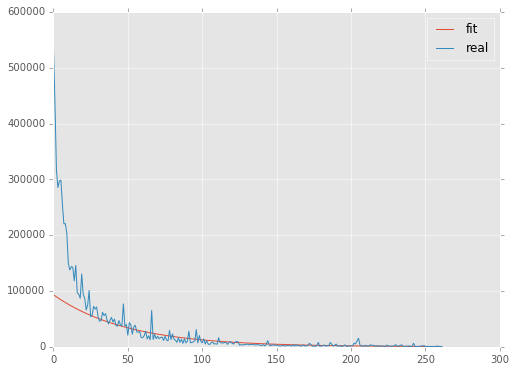
\includegraphics[scale=0.55]{simple-fit.png}

Since the fitting is dominated by the tail data, the rift implies that our model is too weak to express 
the mechanism behind the data.

We can verify this by to regress data chunks separately, 
obviousily if the model is true, $\hat{p}$ will only change little subject to random noise. 
Below results are obtained by taken first $1/10$ data and last $9/10$ data separately:

\[
\hat{p_1} = 0.9275 \quad \hat{p_2} = 0.9824
\]

% Let us merge the two fitting result into a unique figure:





\section{Motivation}

Motivation content.

\end{document}